\section{Introduction}
\label{sec:intro}


On-policy distillation (OPD) has rapidly become a standard component of LLM post-training \citep{gu2024minillm,agarwal2024gkd,song2026survey}. By grounding supervision in student-generated trajectories, OPD mitigates the exposure bias of supervised fine-tuning (SFT) and classical off-policy distillation \citep{bengio2015scheduled,hinton2015distilling,deepseekr1}, while providing dense token-level feedback compared to sparse-reward reinforcement learning (RL). These advantages have made OPD a widely adopted bridge between SFT and RL in modern post-training~\cite{qwen3,glm5,deepseekv4,mimo_v2_flash}.

\begin{figure}[t]
  \centering
  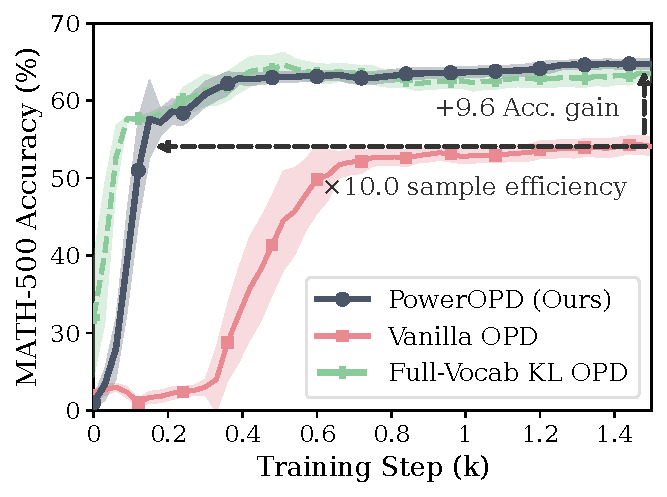
\includegraphics[width=\columnwidth]{figures/fig1_sample_efficiency.pdf}
  \vspace{-20pt}
\caption{PowerOPD achieves $\mathbf{+9.6}$ accuracy gain and $\mathbf{10\times}$ sample efficiency over vanilla OPD, matching or exceeding full-vocabulary KL OPD at 59.2\% less wall-clock time (Qwen3-1.7B $\leftarrow$ Qwen3-4B, \textsc{MATH-500}).}
    \vspace{-5pt}
  \label{fig:first_page}
\end{figure}

In its original form, OPD minimizes the reverse-KL divergence between teacher and student distributions by comparing probabilities over the full vocabulary at each generation step. However, computing the full-vocabulary objective is expensive in practice. Consequently, modern implementations estimate the objective using student-sampled tokens, yielding an unbiased single-sample Monte Carlo estimator \citep{kevin2025opd,jin2026entropy,ko2026reopold,jia2026asymmetric,liu2026teacherguidedpolicyoptimizationonpolicy,zhao2026decouplingkltrajectoriesunified,zhao2026opdrethinkingadvantagedesign}\footnote{As this sampled-token formulation has become the de facto implementation of OPD due to its substantially lower cost, we refer to it as \emph{vanilla OPD} throughout this paper.}.
% This sampled-token approximation preserves OPD's core advantages: 
%This estimator preserves OPD’s core advantages:
%mitigating the exposure bias of supervised fine-tuning (SFT) and classical off-policy distillation \citep{hinton2015distilling,deepseekr1} by grounding supervision in the student's own trajectories \citep{bengio2015scheduled}, while providing denser, token-level feedback compared to sparse outcome-reward reinforcement learning (RL). Consequently, recent industrial pipelines widely adopt OPD as a compute-efficient bridge between SFT and RL \citep{qwen3,glm5,deepseekv4,mimo_v2_flash}.


% Despite its widespread adoption and computational benefits, we identify severe training pathologies that consistently emerge from this sampled-token approximation. In a representative Qwen3-4B teacher and Qwen3-1.7B-Base student setting on \textsc{MATH-500}, it exhibits: (i)~\emph{sample inefficiency}, where validation accuracy initially decreases and does not recover for hundreds of training steps despite dense token-level supervision; (ii)~\emph{unstable generation dynamics}, where response length undergoes large oscillations before stabilizing, indicating that the student repeatedly enters unstable generation regimes; and (iii)~\emph{a substantial gap to full-vocabulary OPD}, where sampled-token OPD plateaus at 54.93\% accuracy, while full-vocabulary OPD reaches 63.12\%, leaving an 8.19-point gap.
Despite its widespread adoption, we observe that vanilla OPD exhibits severe \emph{pathological training dynamics} in practice. In a representative Qwen3-4B teacher and Qwen3-1.7B-Base student setting on \textsc{MATH-500}, validation accuracy initially decreases and does not recover for hundreds of training steps despite dense token-level supervision, indicating sample inefficiency. Meanwhile, response length undergoes large oscillations before stabilizing, indicating that the student repeatedly enters unstable generation regimes. Even after convergence, vanilla OPD reaches only 54.93\% accuracy, trailing full-vocabulary OPD by 8.19 points. Together, these failures suggest that \emph{the Monte Carlo approximation underlying vanilla OPD introduces optimization difficulties that significantly limit both training efficiency and final performance}.

% To understand why vanilla OPD fails, we closely examine the reward signal that directly weights each policy-gradient update: the teacher–student log-probability ratio. Our diagnosis reveals that the unbounded nature of this log-ratio drives the observed training pathologies through three distinct mechanisms:
To understand the source of these pathological training dynamics, we examine the token-level reward that directly weights each policy-gradient update: the teacher-student log-probability ratio. Our diagnosis shows that the unbounded log-ratio reward distorts the update signal along three dimensions:
(i) extreme reward variance, where reward values plummet to nearly $-50$, allowing single rare tokens to dominate gradient updates and trigger generative instability; (ii) early-position extremes, where massive reward magnitudes disproportionately hit the early positions of student rollouts, destabilizing the prefix distribution and causing cascading errors that drive sample inefficiency; and (iii) persistent extreme rewards, where these massive positive and negative values fail to decay, injecting instability throughout the entire optimization process. Notably, applying standard RL reward-stabilization tools \citep{mnih2015human,schulman2017ppo}, such as clipping, tanh compression, and z-score normalization, does not resolve these issues, indicating that \textit{the instability originates from the unbounded log-ratio reward itself rather than from insufficient post-hoc scaling}.

Recognizing that unboundedness is the root cause, we reframe OPD reward design as learning a principled probability-to-reward mapping. A well-conditioned OPD reward must satisfy two properties: boundedness, to prevent rare Monte Carlo events from inducing catastrophic gradient updates, and sign consistency, to ensure the reward sign correctly aligns with the teacher–student probability gap (i.e., yielding a positive reward when the teacher assigns a higher probability than the student, and vice versa). We retain the transform-then-subtract structure of the standard reward, \(h(\pi_T)-h(\pi_\theta)\) because it guarantees sign consistency for any strictly increasing \(h\). To achieve boundedness without losing this directional signal, we instantiate \(h\) using the Box–Cox power family \citep{boxcox1964}. This yields \textbf{PowerOPD}: a family of bounded and sign-consistent OPD rewards parameterized by \(\alpha>0\). While the unstable standard log-ratio reward represents the degenerate \(\alpha\to0\) limit, our formulation ensures the reward remains strictly bounded for any \(\alpha>0\).

We evaluate PowerOPD on six mathematical reasoning benchmarks across four teacher--student pairs from the Qwen3 family (0.6B and 1.7B students; 4B and 8B teachers).
As shown in Figure~\ref{fig:first_page}, using a Qwen3-1.7B-Base student and Qwen3-4B teacher, PowerOPD achieves a $\mathbf{+9.6}$ accuracy gain over vanilla OPD and reaches the same accuracy level with $\mathbf{10\times}$ fewer training steps.
% In full benchmark evaluations across all configurations, PowerOPD improves over vanilla OPD by $\mathbf{+6.37}$ Avg@8 and $\mathbf{+5.71}$ Pass@8 on average, and consistently outperforms full-vocabulary OPD by $\mathbf{+2.59}$ Avg@8 and $\mathbf{+8.90}$ Pass@8 while reducing wall-clock time per step by 59.2\% and peak GPU memory by 23.1\%.
Across the full benchmark evaluation, PowerOPD achieves benchmark-averaged Avg@8/Pass@8 gains of up to $\mathbf{+6.37/+5.71}$ over vanilla OPD, $\mathbf{+3.01/+3.54}$ over post-hoc stabilization, and $\mathbf{+2.59/+8.90}$ over full-vocabulary OPD, with individual-benchmark gains reaching $\mathbf{+16.75/+15.00}$, $\mathbf{+8.43/+7.50}$, and $\mathbf{+11.60/+25.00}$, respectively, while reducing wall-clock time per step by $59.2\%$ and peak GPU memory by $23.1\%$ relative to full-vocabulary OPD.
% Notably, PowerOPD is scalable with respect to $\alpha$: larger $\alpha$ consistently improves final accuracy and Pass@8, shortens response length, and yields faster convergence and more stable generation dynamics throughout training.
Notably, PowerOPD scales with $\alpha$: larger $\alpha$ generally improves accuracy, shortens responses, and stabilizes training dynamics.
% We further show that this scalability is mechanistically grounded: larger $\alpha$ systematically suppresses reward magnitudes on low-probability tokens, preventing rare Monte Carlo events from dominating policy-gradient updates.
We further show that this scalability is mechanistically grounded: larger $\alpha$ suppresses rewards for tokens that both models assign low probability, while focusing learning on tokens that either the teacher or student considers likely.
% Finally, gradient norm tracking reveals that PowerOPD sustains consistently low gradient norms throughout training, more than $\mathbf{3{,}000\times}$ smaller than the initial spike of vanilla OPD, whereas post-hoc methods only partially mitigate instability.
Finally, gradient tracking shows that PowerOPD keeps norms more than $\mathbf{3{,}000\times}$ below vanilla OPD's initial spike, while post-hoc methods only partially stabilize training.

